\chapter{Ενισχυτική Μάθηση}

\section{Γενικά}
Η ενισχυτική μάθηση (ΕΜ) (\en{Reinforcement Learning (RL)}) είναι είναι ένας γενικός όρος που έχει
δοθεί σε μια οικογένεια τεχνικών στις οποίες ένα σύστημα προσπαθεί να μάθει μέσα από την άμεση αλληλεπίδραση
με το περιβάλλον \cite{aigreek}. Είναι τομέας της τεχνητής νοημοσύνης και, πιο συγκεκριμένα, της μηχανικής μάθησης.

Πιο συγκεκριμένα, η ΕΜ είναι η διαδικασία κατα την οποία ένας πράκτορας (\en{agent}) αλληλεπιδρά με το περιβάλλον του,
και μαθαίνει τι να κάνει, παρατηρώντας τις συνέπειες των πράξεων του.
Ο πράκτορας δεν δίνεται πληροφορίες σχετικά με το ποίες ενέργειες (\en{actions}) να επιλέξει, αλλά πρέπει να
ανακαλύψει ποιες ενέργειες προσφέρουν την μέγιστη ανταμοιβή (\en{reward}), δοκιμάζοντας τες \cite{rlbook}.
Επιπλέον, σε πολλές περιπτώσεις οι ενέργειες του πράκτορα δεν επηρεάζουν μόνο την άμεση ανταμοιβή που θα πάρει,
αλλά και από την ανταμοιβή στην επόμενη κατάσταση, και πιθανώς και όλες τις επόμενες ανταμοιβές. Ετσι,μπορεί να υπάρξουν
καταστάσεις που ο πρακτορας θα πρέπει να θυσιάσει την άμεση ανταμοιβή για να αποκτήσει καλύτερες ανταμοιβές μακροπρόθεσμα.
Σύμφωνα με τα παραπάνω, η ΕΜ στοχεύει να λύσει προβλήματα μέσω τεχνικών
\textit{δοκιμής-και-λάθους \en{(trial-and-error)}} σε περιβάλλοντα με \textit{καθυστερημένες ανταμοιβές}.

Μια κομβική ιδέα, πάνω στην οποία στηρίζεται η ΕΜ, είναι η υπόθεση της ανταμοιβής (\en{reward hypothesis}), η ιδέα ότι κάθε στόχος
μπορεί να εκφραστεί ως η μεγιστοποίηση της αναμενόμενης αξίας του σωρευτικού (\en{cummulative}) αθροίσματος ενός μονοδιάστατου
σήματος. Με απλά λόγια, η υπόθεση θέτει την ιδέα ότι κάθε στόχος μπορεί να εκφραστεί σαν την μεγιστοποίηση μιας ανταμοιβής.
Η ανταμοιβή αυτή δεν χρειάζεται απαραίτητα να είναι θετικός αριθμός, αλλά ακόμα και για αρνητικές τιμές της, συνεχίζουμε να καλούμε
τον όρο ανταμοιβή. Για παράδειγμα, αν ο στόχος είναι η έξοδος από ένα λαβύρινθο, η ανταμοιβή μπορεί να είναι αρνητική σε κάθε βήμα
μέχρι την έξοδο, οπού και γίνεται 0. Τότε ο στόχος τελικά είναι η ελαχιστοποίηση της απόλυτης τιμής της ανταμοιβής, δηλαδή η έξοδος
στα λιγότερα βήματα.

Το πεδίο της ΕΜ έχει τις ρίζες του σε δύο περιοχές. Η πρώτη είναι η συμπεριφορική ψυχολογία, από όπου προέρχεται το
παράδειγμα της δοκιμής-και-λάθους, και η δεύτερη είναι η περιοχή του βέλτιστου ελέγχου, από όπου η ΕΜ δανείζεται
τον μαθηματικό φορμαλισμό (κυρίως τον δυναμικό προγραμματισμό) που υποστηρίζει το πεδίο. Είναι σημαντικό να γνωρίζουμε ότι η ΕΜ
βρίσκεται στην τομή πολλών διαφορετικών επιστημονικών πεδίων, οι οποίοι φαίνονται στο Σχήμα~\ref{fig:faces_rl}\cite{silver2015}.
Όλα αυτά τα πεδία προσεγγίζουν ένα παρόμοιο πρόβλημα, αλλά απο διαφορετική σκοπιά και με διαφορετικές παραμέτρους.

\begin{figure}
    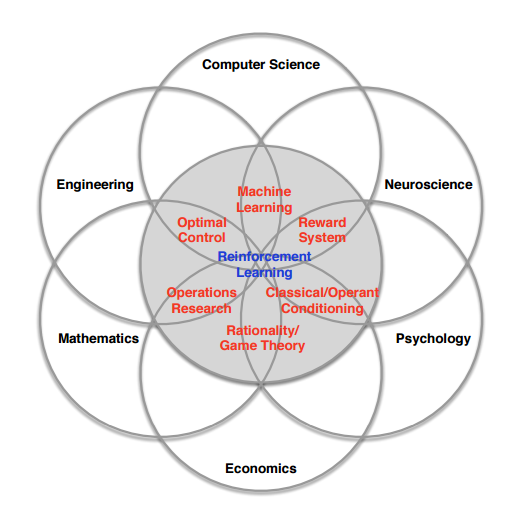
\includegraphics[width=0.5\textwidth]{body_matter/reinforcement_learning/images/faces_of_rl.png}
    \Centering
    \caption{Τα πρόσωπα της ενισχυτικής μάθησης}
    \label{fig:faces_rl}
\end{figure}

Η ΕΜ πολλές φορές συγχέεται με τις άλλες τεχνικές μηχανικής μάθησης, την επιβλεπόμενη και την μη επιβλεπόμενη μάθηση,
παρόλο που έχει αρκετά σημαντικές διαφορές.

Αρχικά, η κύρια διαφορά μεταξύ της επιβλεπόμενης μάθησης (\en{supervised learning}) και της ΕΜ είναι ότι στην επιβλεπόμενη
μάθηση, το μοντέλο εκπαιδεύεται πάνω σε δείγματα (\en{samples}) και ετικέτες (\en{labels}), και κάθε πρόβλεψη θεωρείται
μοναδικό γεγονός. Στόχος είναι η προσέγγιση μιας άγνωστης συνάρτησης με βάση τα δεδομένα.
Αντίθετα, στην ΕΜ, μπορούν να υπάρχουν πολλά βήματα πριν ο πράκτορας μάθει αν η απόφαση που πήρε ήταν
σωστή, και είναι πιθανό να μην μάθει ποτέ ποια ήταν η αληθής/βέλτιστη τιμή. Το μόνο που παρατηρεί είναι η
επίδραση που είχαν οι πράξεις του στο περιβάλλον.

Όσον αφορά την μη επιβλεπόμενη μάθηση, μπορεί αρχικά να φαίνεται παρόμοια με την ΕΜ. Όμως, στόχος της μη επιβλεπόμενης μάθησης
είναι η εύρεση της κρυμμένης δομής δεδομένων τα οποία δεν έχουν ετικέτες. Η ΕΜ έχει διαφορετικό στόχο, ο οποίος είναι η
μεγιστοποίηση του σήματος ανταμοιβής. Παρόλο που η εύρεση δομής είναι πολύ σημαντική και στην ΕΜ ώστε να μπορέσει ο πράκτορας
να επιλέξει τις κατάλληλες κινήσεις, αυτό από μόνο του δεν επιτυγχάνει τον στόχο της ΕΜ.

Ενα από τα κύρια προβλήματα της ΕΜ, που δεν συναντάται στις άλλες μορφές μηχανικής μάθησης είναι
ο συμβιβασμός μεταξύ εξερεύνησης και εκμετάλλευσης. Για να αποκτήσει ο πράκτορας μεγάλη ανταμοιβή
θα προτιμήσει τις ενέργειες που δοκίμασε στο παρελθόν και του προσέφεραν μεγαλύτερη ανταμοιβή. Αλλά
για να ανακαλύψει τέτοιες πράξεις, πρέπει να δοκιμάσει πράξεις που δεν έχει δοκιμάσει στο παρελθόν.
Έτσι ο πράκτορας πρέπει να \textit{εκμεταλλευτεί} το τι έχει ήδη βιώσει ώστε να αποκτήσει ανταμοιβές,
αλλά πρέπει και να \textit{εξερευνήσει}, ώστε να πάρει καλύτερες αποφάσεις στο μέλλον. Έτσι το δίλημμα
είναι ποια από τις δύο στρατηγικές να επιλέξει κάθε φορά, καθώς καμία δεν μπορεί επιδιωχθεί αποκλειστικά,
έτσι ώστε να επιτευχθεί ο στόχος του πράκτορα. Ως αποτέλεσμα, ο πράκτορας πρέπει να δοκιμάσει διάφορες
κινήσεις και προοδευτικά να προτιμήσει αυτές που θεωρεί καλύτερες.Καθώς πολλές από τα προβλήματα που
θέλουμε να λύσουμε με ΕΜ είναι στοχαστικά, ο πράκτορας πρέπει να δοκιμάσει κάθε πράξη πολλές φορές
για να πάρει μια αξιόπιστη εκτίμηση της προσδοκώμενης ανταμοιβής.


\section{Στοιχεία της ΕΜ}

Πέρα από την πράκτορα και το περιβάλλον, υπάρχουν ακόμα τέσσερα κύρια στοιχεία σε ένα σύστημα ΕΜ. Αυτά είναι:
\begin{itemize}
    \item Η πολιτική (\en{policy}), η οποία ορίζει την συμπεριφορά του πράκτορα για μια δοθείσα
          χρονική στιγμη. Με απλά λόγια, η πολιτική είναι μια χαρτογράφηση από τις καταστάσεις
          που αντιλαμβάνεται ο πράκτορας στις ενέργειες που παίρνει σε αυτές τις καταστάσεις (πιο συγκεκριμένα στις πιθανότητες αυτών των ενεργειών). Οι
          πολιτικές μπορεί να είναι και στοχαστικές, προσδιορίζοντας μια πιθανότητα για κάθε ενέργεια.
    \item Το σήμα ανταμοιβής, το οποίο αναφέρθηκε και νωρίτερα. Το σήμα αυτό προσδιορίζει στόχος ενός προβλήματος
          ΕΜ. Σε κάθε χρονικό βήμα, το περιβάλλον στέλνει στον πράκτορα έναν αριθμό, την ανταμοιβή.
          Ο μόνος στόχος του πράκτορα είναι να μεγιστοποιήσει την συνολική ανταμοιβή που λαμβάνει
          μακροπρόθεσμα. Έτσι το σήμα της ανταμοιβής προσδιορίζει	ποιά είναι τα καλά και τα κακά
          γεγονότα για τον πράκτορα. Είναι σημαντικό η ανταμοιβή να προσδιορίζει ακριβώς το
          τι θέλουμε να πετύχουμε. Η ανταμοιβή δεν πρέπει να περιέχει πληροφορίες
          για το πώς θα πετύχουμε τον στόχο. Αυτές οι πληροφορίες μπορούν να τοποθετηθούν μέσα στην πολιτική ή στην συνάρτηση αξίας.
          Το σήμα είναι η κύρια βάση λόγω της οποίας αλλάζει η πολιτική.
          Αν ο πράκτορας επιλέξει μια ενέργεια με μικρή ανταμοιβή, τότε η πολιτική του ίσως να αλλάξει
          για να επιλέξει κάποια άλλη ενέργεια, όταν υπάρξει η ίδια κατάσταση στο μέλλον. Γενικά, οι
          ανταμοιβές μπορεί να είναι στοχαστικές συναρτήσεις της κατάστασης του περιβάλλοντος και των
          ενεργειών που επιλέχθηκαν.
    \item Η συνάρτηση αξίας κάθε κατάστασης \en{(value function)}. Αντίθετα από το σήμα
          ανταμοιβής που μας επιστρέφει το τί είναι καλό άμεσα, η συνάρτηση αξίας προσδιορίζει τι είναι καλό μακροπρόθεσμα. Σε γενικές γραμμές, η αξία μιας κατάστασης είναι η συνολική ανταμοιβή που μπορεί να περιμένει
          να αποκτήσει ένας πράκτορας στο μέλλον, ξεκινώντας από την συγκεκριμένη κατάσταση. Έτσι, ενώ οι ανταμοιβές προσδιορίζουν την άμεση και εσωτερική επιθυμητότητα των καταστάσεων του περιβάλλοντος,
          η αξία υποδεικνύει την μακροπρόθεσμη επιθυμητότητα των καταστάσεων, παίρνοντας υπόψιν τις καταστάσεις
          που θα ακολουθήσουν και τις διαθέσιμες ανταμοιβές σε αυτές τις καταστάσεις. Έτσι, μια κατάσταση
          με χαμηλή ανταμοιβή, μπορεί να έχει μεγάλη αξία γιατί οδηγεί σε καταστάσεις με μεγαλύτερες ανταμοιβές. Ετσι η συνάρτηση αξίας προσδιορίζει πόσο καλό είναι για ένα πράκτορα να είναι στην συγκεκριμένη κατάσταση.
    \item Προαιρετικά,ένα μοντέλο του περιβάλλοντος (\en{model}). Το μοντέλο ενός συστήματος ΕΜ μιμήται την
          συμπεριφορά του συστήματος, ή πιο γενικά, επιτρέπει την δημιουργία συμπερασμάτων για το πώς θα
          συμπεριφερθεί το περιβάλλον. Τα μοντέλα χρησιμοποιούνται για σχεδιασμό \en{(planning)}, δηλαδή την επίλογή της
          σειράς των δράσεων παίρνοντας υπόψιν πιθανές μελλοντικες καταστάσεις, πριν τις βιώσει ο πράκτορας.
          Μέθοδοι επίλυσης προβλημάτων ΕΜ που χρησιμοποιούν μοντέλα και σχεδιασμό λέγονται μέθοδοι βασισμένοι
          σε μοντέλα (\en{model-based}). Αν οι μέθοδοι δεν έχουν μοντέλο, δηλαδή μέθοδοι που μαθαίνουν ρητά μέσω
          δοκιμής-και-λάθους, λέγονται μέθοδοι χωρίς μοντέλο (\en{model-free}).
\end{itemize}

Πιο φορμαλιστικά, σε ένα περιβάλλον ΕΜ, ένας αυτόνομος πράκτορας, ελεγχόμενος από ένα αλγόριθμο μηχανικής μάθησης,
παρατηρεί μια κατάσταση $s_t$ από το περιβάλλον του σε ένα χρονικό βήμα $t$. Οι χρονικές στιγμές στην περιγραφή αυτή είναι διακριτές,
δηλαδή $τ=0,1,2,\ldots$, αλλά θα μπορούσαν να είναι και συνεχείς, χώρις μεγάλες διαφορές. Οι καταστάσεις προέρχονται από τον
χώρο καταστάσεων $\mathcal{S}$. Ο πράκτορας αλληλεπιδρά με το περιβάλλον επιλέγοντας μια ενέργεια $a_t$ με βάση την κατάσταση
$s_t$, επιλεγμένη από ένα χώρο ενεργειών $\mathcal{A}(s)$. Όταν ο πράκτορας εκτελέσει την ενέργεια, τότε τόσο το περιβάλλον,
μεταβαίνει σε μια νέα κατάσταση $s_{t+1}$, με βάση την τρέχουσα κατάσταση και την επιλεγμένη
ενέργεια \cite{drlbs}. Σε κάθε τριπλέτα (κατάστασης, ενέργειας, νέας κατάστασης), αντιστοιχεί μια πιθανότητα μετάβασης
$\Pr{\{S_{t+1}=s'|S_t=s, A_{t}=a\}}$. Σε κάθε κατάσταση,ο πράκτορας μπορεί είναι να παρατηρήσει την πλήρη δυναμική του
περιβάλλοντος ή μέρος της. Ο πράκτορας επίσης λαμβάνει και μια μονοδιάστατη ανταμοιβή $R_t$
η οποία προέρχεται από την τριπλέτα (κατάστασης, ενέργειας, νέας κατάστασης), και συμβολίζεται ως
$R(s_{t-1}, a_{t-1}, s_t)$. Αυτή η ανταμοιβή δεν είναι γνωστή στον πράκτορα στην αρχή και
δρα ως μια μορφή ανατροφοδότησης για τις δράσεις του πράκτορα.
Αυτή η διαδικασία αναπαριστάται οπτικά στο Σχήμα~\ref{fig:agent_environment}.


Συνήθως ο πράκτορας διατηρεί μια εσωτερική κατάσταση, η οποία περιλαμβάνει κομμάτια της κατάστασης του περιβάλλοντος τα οποία θεωρούνται
σημαντικά, καθώς και άλλες πληροφορίες. Σε αυτή την εσωτερική κατάσταση, ο πράκτορας
διατηρεί μια αντιστοίχηση μεταξύ κατάστασης και ενέργειας, η οποία συμβολίζεται ως $\Pr(a_t | s_t)$.

\begin{figure}[ht]
    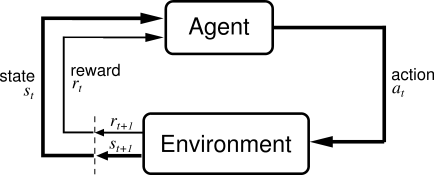
\includegraphics[width=0.5\textwidth]{body_matter/reinforcement_learning/images/agent_environment.png}
    \Centering
    \caption{Αλληλεπίδραση πράκτορα και περιβάλλοντος}
    \label{fig:agent_environment}
\end{figure}


Η βέλτιστη σειρά ενεργειών προσδιορίζεται από τις ανταμοιβές που προμηθεύει το περιβάλλον. Ο τελικός στόχος του πράκτορα είναι να μάθει μια
πολιτική $π$, η οποία μεγιστοποιεί την αναμενόμενη απόδοση (σωρευτική, εκπτωθείσα (\en{discounted}) ανταμοιβή). Δοθείσας μιας κατάστασης
η πολιτική αποφασίζει την επόμενη ενέργεια την οποία θα κάνει ο πράκτορας. Μια βέλτιστη πολιτική είναι η πολιτική η οποία μεγιστοποιεί
την αναμενόμενη απόδοση στο συγκεκριμένο περιβάλλον.

Πέρα απο την περιγραφή του συστήματος ΕΜ με βάση την ύπαρξη ή όχι μοντέλου του περιβάλλοντος, ένας
άλλος τρόπος να περιγράψουμε τα συστήματα ΕΜ είναι με βάση το περιβάλλον στο οποίο βρίσκονται οι πράκτορες. Η μία περίπτωση είναι να είναι αυτό το περιβάλλον πλήρως παρατηρήσιμο, δηλαδή ο πράκτορας μπορεί να παρατηρήσει κάθε πληροφορία για την δυναμική του περιβάλλοντος.
Αυτό φυσικά δεν σημαίνει ότι κάθε παρατήρηση θα είναι χρήσιμη. Έτσι η κατάσταση
του πράκτορα θα είναι το υποσύνολο των παρατηρήσεων που είναι χρήσιμες. Αυτά τα
περιβάλλοντα ικανοποιούν την Μαρκοβιανή ιδιότητα. Δηλαδή, για κάθε κατάσταση, το μέλλον εξαρτάται μόνο από
την τρέχουσα κατάσταση και όχι τις προηγούμενες. Όταν ισχύει αυτή η ιδιότητα τότε μπορούμε να μοντελοποιήσουμε το πρόβλημα ως μια
Μαρκοβιανή Διαδικασία Αποφάσεων (\en{Markov Decision Process}). Αντίθετα, υπάρχουν περιβάλλοντα που δεν είναι πλήρως
παρατηρήσιμα, όπως για παράδειγμα ένα δωμάτιο μέσα στο οποίο κινειται ένα ρομπότ. Σε αυτή την περίπτωση,
το ρομπότ δεν γίνεται σε κάθε κίνηση του να γνωρίζει τα πάντα για το περιβάλλον γιατί υπάρχουν πάρα πολλές παράμετροι.

Η Μαρκοβιανή ιδιότητα ορίζεται ως:
\begin{equation}
    p(r,s|S_t, A_t) = p(r,s | \mathcal{H}_t, A_t)
\end{equation}

το οποίο σημαίνει ότι η πιθανότητα να βρεθούμε στην κατάσταση $s$ με ανταμοιβή $r$, αν γνωρίζουμε
ολόκληρη την ιστορία της αλληλεπίδρασης του πράκτορα με το περιβάλλον και παίρνοντας και κάνοντας
την ενέργεια $A_t$ (αριστερό μέρος) είναι ίδια με την πιθανότητα να βρεθούμε στην κατάσταση $s$ με
ανταμοιβή $r$ γνωρίζοντας μόνο την τελευταία κατάσταση $S_t$ στην οποία βρισκόταν ο πράκτορας
και την ενέργεια $A_t$ που έκανε (δεξί μέρος).

Σε μια Μαρκοβιανή Διαδικασία Αποφάσεων δημιουργούμε μια εκτίμηση της βέλτιστης $q_*(s,α)$ κάθε
ενέργειας $α$ σε κάθε κατάσταση $s$ ή μια εκτίμηση της αξίας $u_*(s)$ κάθε κατάστασης δεδομένης
μιας βέλτιστης επιλογής ενεργειών.

\section{Μαρκοβιανές Διαδικασίες Αποφάσεων}

Για την καλύτερη κατανόηση της ΕΜ, είναι χρήσιμο να περιορίσουμε το πρόβλημα στην μορφή του  που είναι μια ΜΔΑ. Συγκεκριμένα, σε διακριτό χρόνο, η αρχή της πορείας ενός πράκτορα θα είναι

\begin{equation*}
    S_0, A_0, R_1, S_1, A_1, R_2, S_2, A_2
\end{equation*}

Σε μια πεπερασμένη ΜΔΑ, η κατάστασεις, οι ενέργειες και οι ανταμοιβές είναι τα σύνολα
($\mathcal{S}, \mathcal{A}, \mathcal{R}$) με πεπερασμένο αριθμό στοιχείων. Σε αυτή την περίπτωση οι τυχαίες μεταβλητές $R_t$ και $S_t$ έχουν μια καλά ορισμένη διακριτή πιθανότητα, η οποία εξαρτάται από την προηγούμενη κατάσταση και ενέργεια. Έτσι η δυναμική της ΜΔΑ ορίζεται από την συνάρτηση, η οποία λόγω της Μαρκοβιανής ιδιότητας προσδιορίζει πλήρως την δυναμική του συστήματος.
\begin{equation}
    p(s', r | s, a) = \Pr{S_t = s', R_t = r | S_{t-1} = s, A_{t-1} = a }
\end{equation}

Όσον αφορά το σήμα ανταμοιβής, ο στόχος είναι η μεγιστοποίηση του σε βάθος χρόνου. Αυτό αναφέρεται στην βιβλιογραφία ως απόδοση (\en{return}) οπως αναφέρθηκε και νωρίτερα, η οποία πολύ συχνά αναπαριστάται ως $G_t$.

Ανάλογα με το αν τερματίζει ένα πρόβλημα, αυτό μπορεί να θεωρηθεί επεισοδικό ή συνεχές. Σε ένα επεισοδικό πρόβλημα, υπάρχει πάντα μια τελική κατάσταση (π.χ. η έξοδος ενός λαβυρίνθου).
Σε ένα συνεχές πρόβλημα, δεν υπάρχει αυτός ο διαχωρισμός σε επεισόδια, αλλά η αλληλεπίδραση συνεχίζεται ατέρμονα. Για να μπορέσουμε να υπολογίσουμε την απόδοση ακόμα και σε συνεχή προβλήματα, συνήθως την ορίζουμε ως

\begin{equation}
    G_t = R_{t+1} + γ R_{t+2} + γ^2 R_{t+3} + \ldots = \sum_{k=0}^{\infty}γ^k R_{t+k+1}
\end{equation}
όπου $ 0 \leq γ \leq 1$ είναι μια παράμετρος η οποία ονομάζεται παράγοντας έκπτωσης. Ο παράγοντας αυτός επηρεάζει το πόσο σημασία έχουν οι μετέπειτα ανταμοιβές. Επίσης, έχει μαθηματική αξία, καθώς εξασφαλίζει ότι η απόδοση είναι πάντα φραγμένη (για $γ < 1$).

Για $γ = 0$, ο πράκτορας είναι μυοπυκός, δηλαδή ενδιαφέρεται να εξασφαλίσει την καλύτερη ανταμοιβή σε κάθε βήμα, ανεξάρτητα αν αυτό σημαίνει ότι θα χάσει καλύτερες ανταμοιβές αργότερα, ενώ οσο η τιμή πηγαίνει προς το 1, ο πράκτορας βλέπει όλο και πιο μακριά.

Με βάση τα παραπάνω, μπορούμε πλεον να προσδιορίσουμε και πιο φορμαλιστικά την περιγραφή της πολιτικής του πράκτορα και της συνάρτησης αξίας. Οπως αναφέρθηκε ήδη η πολιτική είναι μια αντιστοίχηση μεταξύ καταστάσεων και πιθανοτήτων επιλογής πράξεων. Αν ένας πράκτορας ακολουθεί μια πολιτική $π$ την χρονική στιγμή $t$, τότε $π(a|s)$ είναι η πιθανότητα ότι θα επιλεχθεί $A_t = a$, αν $S_t =s$.

Η συνάρτηση αξίας μιας κατάστασης $s$ όταν ο πράκτορας ακολουθεί μια πολιτική $π$, με ένδειξη $υ_π(s)$ είναι η αναμενόμενη απόδοση όταν ο πράκτορας ξεκινήσει από την κατάσταση $s$ και ακολουθήσει την πολιτική $π$. Για ΜΔΑ, αυτή ορίζεται ως
\begin{equation}
    υ_π(s) = \mathbb{E}_π[G_t\;|\;S_t = s] = \mathbb{E}_π \left[ \sum_{k=0}^{\infty}γ^kR_{t+k+1}\;\bigg|\;S_t = s\right]
\end{equation}
για όλες τις καταστάσεις $s$ του συνόλου $\mathcal{S}$. Το $\mathbb{E}_π[\cdot]$ είανι η αναμενόμενη τιμή μιας τυχαίας μεταβλητής δεδομένου ότι ο πράκτορας ακολουθεί πολιτική $π$ και $t$ είναι το χρονικό βήμα. Αυτή η συνάρτηση παραπάνω ορίζεται ως συνάρτηση αξίας-κατάστασης για την πολιτική $π$.

Μπορούμε να ορίσουμε και την συνάρτηση αξίας-ενέργειας για την πολιτική $π$, η οποία ορίζεται ως
\begin{equation}
    q_π(s,a) = \mathbb{E}_π[G_t | S_t = s, A_t = a] = \mathbb{E}_π\left[ \sum_{k=0}^{\infty} γ^k R_{t+k+1} \bigg| S_t = s, A_t = a\right]
\end{equation}
η οποία προσδιορίζει την αξία του να κανει ο πράκτορας της ενέργεια $a$ στην κατάσταση $s$ υπο την πολιτική $π$, η οποία είναι η αναμενόμενη απόδοση που θα έχει ο πράκτορας αν στην κατάσταση $s$ κάνει την ενέργεια $a$ και μετά συνεχίσει με την πολιτική $π$.

Οι δύο συναρτήσεις αξίας, μπορούν να υπολογιστούν με βάση την εμπειρία που αποκτά ο πράκτορας κατά την μετάβαση του μεταξύ των καταστάσεων. Για παράδειγμα αν ακολουθεί την πολιτική $π$, τότε για κάθε κατάσταση, όσο πιο συχνά την επισκέφτεται, τόσο πιο κοντά θα φτάνει η μέση τιμή στην πραγματική αξία $υ_π(s)$ της κατάστασης. Αντίστοια αν κρατάει μέσους όρους για κάθε πράξη σε κάθε κατάταση, θα φτάσει στην πραγματική αξία $q_π(s,a)$ της δράσης. Οι τεχνικές αυτές ονομάζονται Μόντε Κάρλο, γιατί βρίσκουν μέσους όρους πολλών τυχαίων δειγμάτων πραγματικών αποδόσεων. Ένας άλλος τρόπος είναι με χρήση συναρτήσεων που προσομοιώνουν τις συναρτήσεις αξιών, και είναι χρήσιμες όταν υπάρχει πολύ μεγάλος αριθμός καταστάσεων και η αποθήκευση όλων των τιμών δεν είναι δυνατή.

Στόχος της ΕΜ είναι η εύρεση βέλτιστων πολιτικών που θα επιφέρουν μεγάλη ανταμοιβή μακροπρόθεσμα. Σε πεπερασμένες ΜΔΑ η βέλτιστη απόφαση είναι πλήρως ορισμένη, και είναι η πολιτική που επιφέρει μεγαλύτερη ή ίση αξία με όλες τις υπόλοιπες πολιτικές. Αυτή η βέλτιστη πολιτική, δεν είναι να βρεθεί σε πραγματικά προβλήματα, γιατί
\begin{enumerate}
    \item η δυναμική του περιβάλλοντος δεν είναι γνωστή ακριβώς,
    \item δεν είναι υπολογιστικά εφικτό να υπολογιστεί η βέλτιστη πολιτική, πχ γιατί ο χώρος καταστάσεων είναι τεράστιος,
    \item οι καταστάσεις δεν έχουν την Μαρκοβιανή ιδιότητα.
\end{enumerate}

Σε αυτές τις περιπτώσεις, η μόνη μας επιλογή είναι είτε να δημιουργήσουμε προσεγγίσεις της βέλτιστης πολιτικής ή να χρησιμοποιήσουμε ευριστικές, ή και τα δύο.

\section{Συμπεράσματα}

Το πρόβλημα της Ενισχυτικής Μάθησης, μελετάει την έυρεση βέλτιστων πολιτικών για πράκτορες που κινούνται μέσα σε ένα περιβάλλον, πολιτικών δηλαδή που προσφέρουν την μέγιστη αξία στον πράκτορα. Επειδή πολλές η εύρεση της βέλτιστης πολιτικής δεν είναι πρακτικά δυνατή, χρησιμοποιούμε προσεγγίσεις και ευριστικές.

Στην δική μας εργασία, οι καταστάσεις του περιβάλλοντος είναι γνωστές και πεπερασμένες, και φραγμένες από τον αριθμό των θεμάτων που μπορεί να συζητήσει ο πράκτορας μας, οι οποίες δεν είναι πάρα πολλές. Επιπλέον, μπορούμε να θεωρήσουμε ότι οι καταστάσεις έχουν την Μαρκοβιανή ιδιότητα, καθώς η τρέχουσα κατάσταση μπορεί να περιλαμβάνει χαρακτηριστικά του διαλόγου του πράκτορα με τον χρήστη. Το πρόβλημα είναι ότι οι δυναμικές του συστήματος είναι πλήρως άγνωστες και μεταβλητές, καθώς δεν γνωρίζουμε καμία πληροφορία για τον χρήστη κατα την αρχή της συζήτησης για να μπορέσουμε να επιλέξουμε σωστά προτάσεις, και επιπλέον τα ενδιαφέροντα των χρηστών στο σύνολο μετακινούνται με την πάροδο του χρόνου. Επειδή ο συγκεκριμένος πράκτορας δεν αποκτά πολλές πληροοφορίες για το περιβάλλον, καθώς δεν υπάρχουν πολλοί χρήστες, θα πρέπει να απλοποιήσουμε το πρόβλημα και να μην ασχοληθούμε με το πλήρες πρόβλημα της ενισχυτικής μάθησης, αλλά με ένα πιο περιορισμένο, το πρόβλημα των \en{bandits}.
